\documentclass[12pt,oneside]{report}
\usepackage[a4paper,left=4.2cm,right=2.5cm,top=2.85cm,bottom=2.85cm,headheight=16pt,headsep=18pt,footskip=30pt]{geometry}
\usepackage{fontspec}\setmainfont{Times New Roman}
\usepackage{tabularx}
\usepackage{graphicx,setspace,titlesec,tocloft,array,booktabs,longtable,enumitem,amsmath,caption,xcolor,listings,float,tikz,atbegshi,eso-pic,ragged2e,placeins,fancyhdr,draftwatermark}
\floatplacement{figure}{H}
\floatplacement{table}{H}
\usetikzlibrary{positioning,arrows.meta,shapes.geometric,calc,fit,backgrounds}
\usepackage[hidelinks]{hyperref}
\onehalfspacing\setlength{\emergencystretch}{3em}\captionsetup{font=small,labelfont=bf,skip=6pt}
\let\oldunderscore\_\renewcommand{\_}{\oldunderscore\allowbreak}
\renewcommand{\topfraction}{0.9}\renewcommand{\bottomfraction}{0.8}\renewcommand{\textfraction}{0.07}\renewcommand{\floatpagefraction}{0.75}
\titleformat{\chapter}[display]{\normalfont\fontsize{16}{19}\bfseries\centering}{Chapter \thechapter}{1ex}{\MakeUppercase}\titlespacing*{\chapter}{0pt}{-10pt}{20pt}
\titleformat{\section}{\normalfont\fontsize{14}{17}\bfseries}{\thesection}{0.6em}{}\titlespacing*{\section}{0pt}{18pt}{10pt}
\titleformat{\subsection}{\normalfont\fontsize{14}{17}\bfseries}{\thesubsection}{0.6em}{}\titlespacing*{\subsection}{0pt}{10pt}{6pt}
\newcommand{\ProjTitle}{Explainable AI Text Detection}
\pagestyle{fancy}\fancyhf{}\fancyhead[L]{\textit{\ProjTitle}}\fancyhead[R]{2026--2027}\fancyfoot[L]{Department of AIML, RVCE}\fancyfoot[R]{\thepage}\fancyheadoffset[L]{0cm}\fancyheadoffset[R]{0cm}\fancyfootoffset[L]{0cm}\fancyfootoffset[R]{0cm}\renewcommand{\headrulewidth}{0pt}\renewcommand{\footrulewidth}{0pt}
\fancypagestyle{plain}{\fancyhf{}\fancyhead[L]{\textit{\ProjTitle}}\fancyhead[R]{2026--2027}\fancyfoot[L]{Department of AIML, RVCE}\fancyfoot[R]{\thepage}\renewcommand{\headrulewidth}{0pt}\renewcommand{\footrulewidth}{0pt}}
\fancypagestyle{front}{\fancyhf{}\fancyfoot[R]{\thepage}\renewcommand{\headrulewidth}{0pt}\renewcommand{\footrulewidth}{0pt}}
\newcommand{\PageBorder}{%
  \begin{tikzpicture}[overlay,remember picture]
    \draw[line width=1pt]
      ([shift={(3.51cm,-2.24cm)}]current page.north west)
      rectangle
      ([shift={(-1.8cm,2.24cm)}]current page.south east);
  \end{tikzpicture}%
}
\AddToShipoutPictureFG{\PageBorder}
\SetWatermarkText{
\includegraphics[width=8cm]{logo.png}}\SetWatermarkScale{1}\SetWatermarkAngle{0}\SetWatermarkColor[gray]{0.9}\SetWatermarkHorCenter{11.355cm}\SetWatermarkVerCenter{14.85cm}
\definecolor{codebg}{rgb}{0.96,0.96,0.98}\lstdefinestyle{code}{backgroundcolor=\color{codebg},basicstyle=\ttfamily\scriptsize,breaklines=true,frame=single,columns=fullflexible,keepspaces=true}\lstset{style=code}
\graphicspath{{../outputs/figures/}}
\newcommand{\auditfigure}[3]{\begin{figure}[htbp]\centering\includegraphics[width=#1\linewidth]{#2}\caption{#3}\end{figure}}
\begin{document}
\pagenumbering{roman}
\setcounter{page}{1}
\pagestyle{fancy}
\begin{titlepage}
\thispagestyle{empty}
\SetWatermarkText{
\includegraphics[width=8cm]{logo.png}}

\begin{center}
\begin{tabular*}{\textwidth}{@{\extracolsep{\fill}}lr}
\begin{tabular}[c]{l}\hspace*{-0.9cm}
\includegraphics[width=7.5cm]{front_header.png}\end{tabular}
&\begin{tabular}[c]{r}{\fontsize{19}{23}\selectfont\textit{Go, change the world}}\end{tabular}
\end{tabular*}\\[0.35cm]

{\fontsize{18}{21}\selectfont\textcolor{red}{\textbf{DEPARTMENT OF}}}\\[0.1cm]
{\fontsize{15}{18}\selectfont\textcolor{red}{\textbf{ARTIFICIAL INTELLIGENCE AND MACHINE LEARNING}}}\\[0.25cm]
{\small Bengaluru -- 560059}\\[0.75cm]

{\fontsize{17}{21}\selectfont\textbf{Explainable Evaluation of}}\\[0.15cm]
{\fontsize{17}{21}\selectfont\textbf{AI-Generated Text Detection}}\\[0.35cm]

{\normalsize\textbf{By}}\\[0.2cm]
{\normalsize\textbf{Project Report}}\\[0.25cm]
{\normalsize\textbf{Submitted by}}\\[0.25cm]

{\fontsize{12}{15}\selectfont
\begin{tabular}{ll}
\textbf{NAME OF THE CANDIDATE(S)} & \textbf{USN} \\
To be supplied & To be supplied
\end{tabular}}\\[0.7cm]

{\normalsize in partial fulfillment for the requirement of 7\textsuperscript{th} Semester}\\[0.15cm]
{\normalsize\textbf{Course and code to be supplied}}\\[0.35cm]

{\normalsize\textbf{Under the Guidance of}}\\[0.25cm]
\begin{tabular*}{0.95\textwidth}{@{\extracolsep{\fill}}cc}
\textbf{To be supplied} & \textbf{To be supplied} \\
Associate Professor & Associate Professor \\
Department of AIML & Department of AIML \\
RV College of Engineering & RV College of Engineering \\
Bengaluru--59 & Bengaluru--59
\end{tabular*}\\[0.35cm]

{\normalsize\textbf{Academic Year}}\\[0.1cm]
{\normalsize\textbf{2026 -- 2027}}
\end{center}

\end{titlepage}
\SetWatermarkText{
\includegraphics[width=8cm]{logo.png}}
\clearpage
\ClearShipoutPictureFG
\thispagestyle{empty}\null\clearpage
\AddToShipoutPictureFG{\PageBorder}
\newpage
\cleardoublepage
\pagestyle{empty}
\thispagestyle{empty}

\begin{center}
{\Large\textbf{RV COLLEGE OF ENGINEERING\textsuperscript{\textregistered}}}\\[0.25cm]
{\small (Autonomous Institution Affiliated to Visvesvaraya Technological University, Belagavi)}\\[0.7cm]
{\Large\textbf{DEPARTMENT OF ARTIFICIAL INTELLIGENCE}}\\[0.15cm]
{\Large\textbf{AND MACHINE LEARNING}}\\[0.25cm]
{\small Bengaluru -- 560059}\\[1cm]

\includegraphics[width=3.0cm]{rvlogo.png}\\[0.9cm]
{\Large\underline{\textbf{CERTIFICATE}}}\\[0.6cm]
\end{center}

\begin{center}
\begin{minipage}{1.0\textwidth}
\justifying
\noindent
Project title: \textbf{Explainable AI Text Detection}. Candidate names, USNs, course details, and approval are to be completed by the department before signing.
\end{minipage}
\end{center}

\vspace{1.5cm}
\begin{center}
\begin{tabular*}{\textwidth}{@{\extracolsep{\fill}}cc}
\begin{tabular}[t]{c}
\textbf{Signature of Faculty In-charge}\\
\textbf{Dept. of AIML, RVCE}
\end{tabular}
&
\begin{tabular}[t]{c}
\textbf{HoD}\\
\textbf{Dept. of AIML, RVCE}
\end{tabular}
\end{tabular*}

\vspace{1cm}
\noindent
\textbf{\underline{External Examination}}

\begin{tabular*}{\textwidth}{@{\extracolsep{\fill}}ll}
\textbf{Name of Examiners} &
\textbf{Signature with date} \\
\textbf{1} & \\[0.25cm]
\textbf{2} &
\end{tabular*}
\end{center}
\vfill

\thispagestyle{empty}

\clearpage
\ClearShipoutPictureFG
\thispagestyle{empty}\null\clearpage
\AddToShipoutPictureFG{\PageBorder}

\chapter*{Abstract}
\addcontentsline{toc}{chapter}{Abstract}
\begingroup
\setlength{\parskip}{0.45em}
We audit a pretrained random forest on a balanced sample of 10,000 English records from RAID, the Robust AI Detection benchmark. The classifier uses eight stylometric inputs and achieves 60.99\% accuracy. Its 2,296 false positives and 1,605 false negatives motivate analyses of feature sensitivity, local attribution, stability, calibration, and performance across groups. The resulting presentation delivers recorded model evidence in a reproducible static website.

\par
\endgroup
\clearpage
\ClearShipoutPictureFG
\thispagestyle{empty}\null\clearpage
\AddToShipoutPictureFG{\PageBorder}
\tableofcontents\thispagestyle{fancy}
\clearpage
\listoftables\addcontentsline{toc}{chapter}{List of Tables}
\clearpage
\listoffigures\addcontentsline{toc}{chapter}{List of Figures}
\clearpage
\pagenumbering{arabic}\pagestyle{fancy}

\chapter{Introduction}
\section{Project Description}
Text detectors make probabilistic judgments about writing. This project investigates the behavior and limitations of a frozen stylometric classifier using InterpretML. The same feature pipeline supports the performance evaluation and all model explanations.
\section{Report Organization}
Chapters 2--4 describe the problem, objectives, and techniques. Chapters 5--6 trace the architecture and evidence. Chapters 7--8 summarize the findings and identify further experiments.
\chapter{Problem Definition}
\section{Problem Statement}
Determine how a fixed classifier responds to changes in text statistics and assess how its scores and attributions behave across the benchmark. The balanced evaluation cohort has 5,000 human and 5,000 AI records. Calibration estimates describe this sampling design.
\section{Literature Review}
RAID evaluates detectors across generators, domains, attacks, and decoding strategies \cite{raid}. M4 studies cross-domain and cross-generator generalization \cite{m4}. Kernel SHAP estimation introduces sampling choices that can affect attribution stability \cite{kernel}. The project bibliography records 25 post-2020 studies with relevance notes and publication links.
\chapter{Objectives}
\begin{enumerate}
\item Reproduce the published confusion matrix using the exact sample IDs and frozen artifact.
\item Compare global sensitivity, population-average response, and local attribution.
\item Assess attribution repeatability, score calibration, and threshold trade-offs.
\item Surface benchmark slices and representative cases through a deployable presentation.
\end{enumerate}
\chapter{Tools and Techniques Used}
Python in a project-local virtual environment runs feature extraction, scikit-learn inference, InterpretML, and artifact export. JavaScript reads the resulting JSON and CSV. GitHub Pages hosts the presentation.
\begin{table}[htbp]\centering
\caption{Methods and the questions they answer}
\begin{tabularx}{\linewidth}{lX}
\toprule Method & Evidence produced \\ \midrule
Pearson correlation & Linear associations among inputs in the 500-row PDP cohort. \\
Morris & Global sensitivity to changes in an input. \\
PDP & Mean AI score over a background sample at each feature setting. \\
LIME & Signed coefficients from a local approximation. \\
Kernel SHAP & Signed contributions relative to a background expectation. \\
What-if & Recorded change in one case after replacing one feature. \\
\bottomrule
\end{tabularx}
\end{table}
\chapter{Implementation}
\section{High-level architecture}
\begin{figure}[htbp]\centering
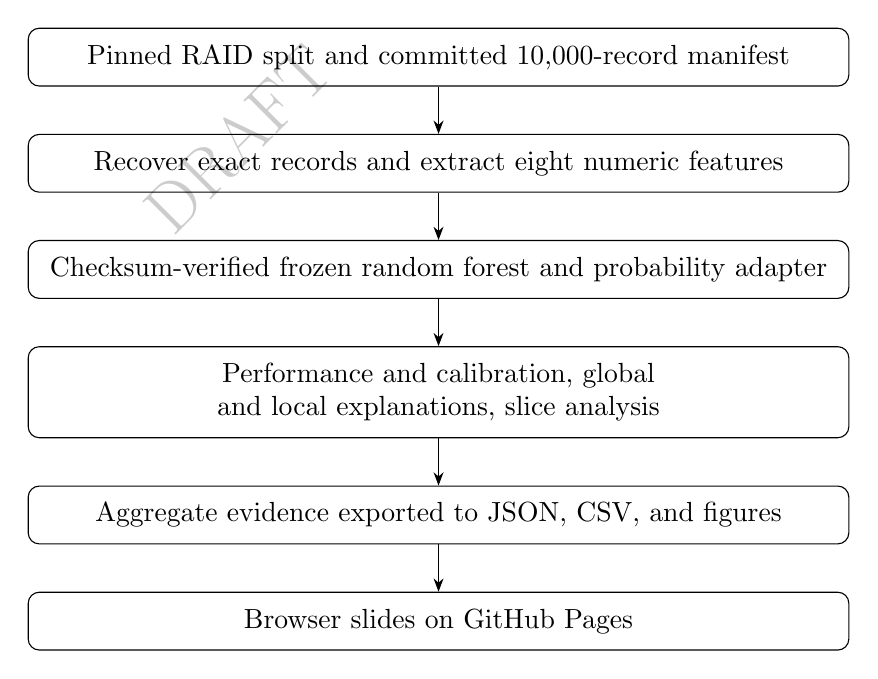
\begin{tikzpicture}[node distance=6mm, box/.style={draw, rounded corners, align=center,text width=10cm,inner sep=6pt}, flow/.style={-{Stealth}}]
\node[box] (data) {Pinned RAID split and committed 10,000-record manifest};
\node[box,below=of data] (features) {Recover exact records and extract eight numeric features};
\node[box,below=of features] (model) {Checksum-verified frozen random forest and probability adapter};
\node[box,below=of model] (audit) {Performance and calibration, global and local explanations, slice analysis};
\node[box,below=of audit] (export) {Aggregate evidence exported to JSON, CSV, and figures};
\node[box,below=of export] (pages) {Browser slides on GitHub Pages};
\draw[flow] (data)--(features); \draw[flow] (features)--(model); \draw[flow] (model)--(audit);
\draw[flow] (audit)--(export); \draw[flow] (export)--(pages);
\end{tikzpicture}
\caption{End-to-end experiment and publishing architecture}
\end{figure}
\section{Data and model contracts}
The ordered features are character count, word count, average word length, punctuation count, sentence count, average sentence length, uppercase word count, and title-case word count. The model has 100 trees. The probability adapter forwards numeric feature vectors to the frozen classifier. Class 0 is Human and class 1 is AI.
\section{Reproducibility and publication}
The sample recovery matches published IDs against the pinned dataset. The audit export checks the confusion matrix against the original evaluation. The local environment and recovered text are excluded from Git. The deployed deck loads precomputed evidence.
\chapter{Results and Discussion}
\begin{table}[htbp]\centering
\caption{Frozen-model results on the exact RAID sample}
\begin{tabular}{lr}\toprule Measure & Value \\ \midrule
Accuracy & 60.99\% \\
AI precision & 59.66\% \\
AI recall & 67.90\% \\
ROC-AUC & 0.645 \\
Brier score & 0.2890 \\
Ten-bin expected calibration error & 21.02\% \\
False positives & 2,296 \\
False negatives & 1,605 \\ \bottomrule
\end{tabular}\end{table}
\auditfigure{0.67}{confusion_matrix.png}{Confusion matrix. Rows are actual classes and columns are predictions.}
\section{Correlation and global model behavior}
Character and word count have a Pearson correlation of 0.91. Word and sentence count have a correlation of 0.84. These relationships can complicate interpretation when one feature changes independently. Morris ranks average word length highest. PDP shows the average response rather than the response of any one record.
\auditfigure{0.87}{feature_correlation.png}{Pearson coefficients from the 500 rows used for PDP.}
\auditfigure{0.82}{morris_sensitivity.png}{Measured Morris sensitivity.}
\auditfigure{0.95}{partial_dependence.png}{Partial dependence across the numeric inputs.}
\section{Local stability and error analysis}
Each of the four cases represents one cell of the confusion matrix. Five seeded reruns yielded Stable Kernel SHAP attributions across all four cases and Mixed LIME attributions for two cases. The model probabilities stayed constant. Attribution variability therefore arises even when the prediction is fixed.

The slice explorer compares mean absolute Kernel SHAP values with a common reference background and up to 24 explained records per group. It reports group sizes and allows comparisons by domain, generator, attack status, decoding, repetition penalty, and true class. These summaries describe the sampled groups and support hypothesis generation. They cannot isolate the effect of a single metadata field.
\section{Calibration and threshold choice}
\auditfigure{1.0}{calibration.png}{Reliability by score bin and score distributions by actual class.}
At the evaluated decision rule, AI scores strictly greater than 0.50 are flagged. Moving the threshold changes both kinds of error. The Brier score measures mean squared probability error, while expected calibration error summarizes the sample-weighted gap between mean scores and observed rates across bins.
\chapter{Conclusion}
The frozen classifier makes substantial errors on the matched RAID cohort. Correlation, Morris, PDP, local attributions, stability checks, and calibration each illuminate a different aspect of its behavior. Detector scores alone cannot establish authorship.
\chapter{Future Enhancements}
Use stratified bootstrap intervals, compare calibration across independent samples with different class prevalence, and test attribution sensitivity to background choice. Evaluate grouped perturbations for correlated features and document their effects on explanation fidelity.
\begin{thebibliography}{9}
\bibitem{raid} L. Dugan et al. RAID: A Shared Benchmark for Robust Evaluation of Machine-Generated Text Detectors. ACL, 2024. \url{https://aclanthology.org/2024.acl-long.674/}
\bibitem{m4} Y. Wang et al. M4: Multi-generator, Multi-domain, and Multi-lingual Black-Box Machine-Generated Text Detection. EACL, 2024. \url{https://aclanthology.org/2024.eacl-long.83/}
\bibitem{kernel} I. Covert and S.-I. Lee. Improving KernelSHAP: Practical Shapley Value Estimation Using Linear Regression. AISTATS, 2021. \url{https://proceedings.mlr.press/v130/covert21a.html}
\end{thebibliography}
\end{document}
